\documentclass[12pt]{article}
\usepackage{graphicx}
\graphicspath{{imgs/}}
\usepackage{xeCJK}
\setCJKmainfont{Noto Serif CJK TC}
\usepackage[top=2cm, bottom=2cm, left=2cm, right=2cm, a4paper]{geometry}
\usepackage{setspace}
\setlength{\parskip}{2pt}
\usepackage{moresize}
\usepackage{placeins}
\usepackage{xcolor}
\usepackage{minted}
\usemintedstyle{fruity}
\usepackage{amsmath}
\usepackage{caption}
\usepackage{subcaption}

\begin{document}

\begin{center}
    \huge \textbf{EDA Final Project Report}
    
    \vspace{10pt}
    
    \large \textbf{110511010 楊育陞 110511067 葉哲伍}
\end{center}

\section{ICCAD 繳交截圖}

\section{Introduction}
We take the \textbf{problem B} of the ICCAD contest as our final project. The problem is "Power and Timing Optimization Using Multibit Flip-Flop". Our method to solve this problem is mainly based on \textbf{clustering} and \textbf{gain-based greedy algorithm}. The clustering algorithm we use is inspired by the "Effective Mean Shift Algorithm" described in the paper "Graceful Register Clustering by Effective Mean Shift Algorithm for Power and Timing Balancing" \cite{jiang}.

\section{Method}

\subsection{Flowchart}

\begin{figure}[htbp]
    \centering
    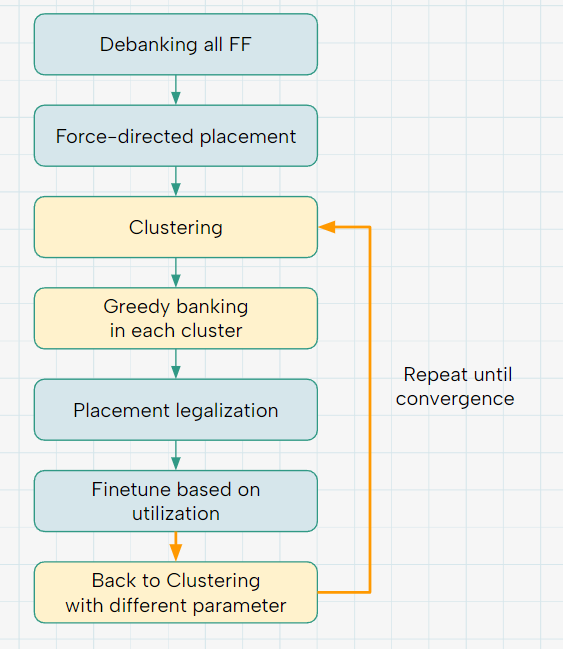
\includegraphics[width=0.7\textwidth]{flowchart.png}
    \caption{Flowchart of our method}
    \label{fig:flowchart}
\end{figure}
\FloatBarrier

\subsection{Division of Labor}
\begin{itemize}
    \item 楊育陞: Debanking, Greedy banking, Finetuning based on utilzation
    \item 葉哲伍: Force-directed placement, Clustering, Placement legalization
\end{itemize}

\subsection{Detailed Explanation}

Our flow of the method is shown in Figure \ref{fig:flowchart}. We will explain each step in detail in the following subsections.

\subsubsection{Debanking all flip-flops}

\subsubsection{Force-directed placement}

\subsubsection{Clustering}

\subsubsection{Greedy banking in each cluster}

\subsubsection{Placement legalization}

\subsubsection{Finetuning based on utilization}

\subsubsection{Back to clustering with different parameters}

\section{Result}

\section{Conclusion}

\begin{thebibliography}{9}
    \bibitem{jiang} 
    Ya-Chu Chang, Tung-Wei Lin, Iris Hui-Ru Jiang, and GiJoon Nam. "Graceful Register Clustering by Effective Mean Shift Algorithm for Power and Timing Balancing." Proceedings of the 2019 International Symposium on Physical Design (ISPD '19), 2019.
\end{thebibliography}

\end{document}
